\subsection{Integration time and approximation error}
We fixed the witness matrix to compare integration algorithms independently of neighbour search and model fitting. For each width $p\in\{64,512,4096,16384\}$, we generated 192 triplets under two abstention probabilities, 0.1 and 0.8, using three seeds per setting. Before abstention, a ballot was positive with probability equal to the logistic function of a Gaussian row effect plus a Gaussian column effect (standard deviations 0.8 and 0.45). Each matrix supplied the exact size minimum, a deterministic computation using independent replacement draws, and Monte Carlo minima at 4, 16, 64 and 256 draws per nonempty layer. The replacement computation propagates the three-outcome margin distribution by convolution. The MC code pools row updates across draws and corrects the focal column when it enters the sampled prefix. Each timing is the median of three single-thread executions in randomized order, following a warm-up.

\begin{figure}[tbp]
\centering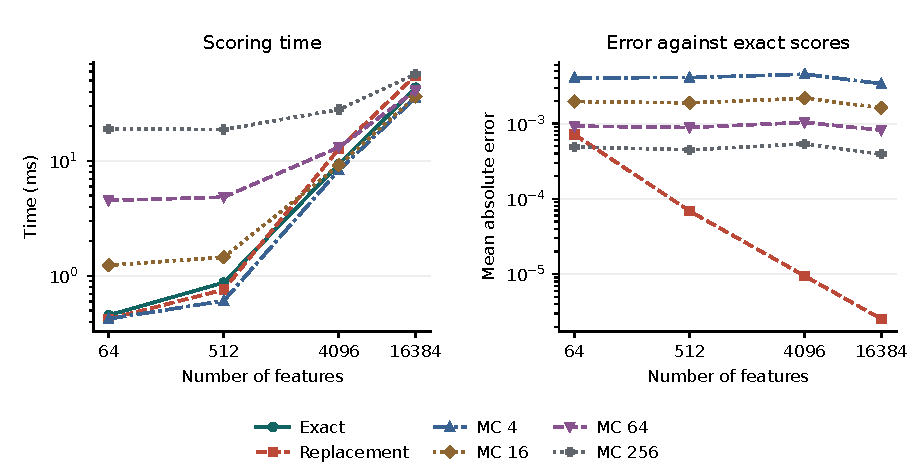
\includegraphics[width=\linewidth]{figures/kernel}
\caption{Computing the size minimum on fixed synthetic vote matrices. Left, median scoring time over six matrices at each width (two abstention rates and three seeds), after taking the median of three runs for each matrix. Right, median across the same six matrices of mean absolute error across columns. MC labels give draws per positive coalition size. Exact counting has zero reference error; its curve is omitted from the logarithmic error axis.}
\label{fig:kernel}
\end{figure}
Across the six matrices at each width, the largest feature-wise replacement error observed fell from 0.00516 at 64 features to 0.0000311 at 16,384, consistent with Theorem~\ref{thm:agreement}. At the largest width the average fraction of the exact top set recovered by four-draw MC was 0.753; at 256 draws it was 0.966. Those fractions count membership in the exact set with the same width, rather than dividing by the union as in Table~\ref{tab:ablation}. At that width median scoring times were 43.4\,ms for exact integration, 35.7\,ms for four draws and 56.9\,ms for 256 draws. Independent replacement gave median mean absolute error $3\times10^{-6}$ in 55.1\,ms (Fig.~\ref{fig:kernel}).
